\newpage
\section{Auswertung}
\subsection{Lorentzfits}
Wie bereits erwähnt, suchten wir die $90^{\circ}$-Einstellung und kalibrierten dann für die $0^{\circ}$-Einstellung die Magnetfelder. Die getroffenen Einstellungen sind dem Anhang $8.1$ zu entnehmen.\\
Mit diesen Einstellungen nahmen wir dann, wie bereits diskutiert, eine Messreihe auf. Für die resultierenden Kurven erfolgte eine Anpassung, wobei die Funktion folgende Form aufwies: \[y(x)=A\cdot\frac{\tau\cdot(2\tau\cdot c(x-x_{0})\sin(2\theta)-\cos(2\theta)+4\tau^{2}c^{2}(x-x_{0})^{2}+1)}{2(4\tau^{2}c^{2}(x-x_{0})^{2}+1)}+y_{0},\] wobei die Kurve für $\theta=0^{\circ}$ in eine normale, für $\theta=90^{\circ}$ in eine invertierte Lorentzkurve übergeht. Den Parametern kommen dabei in ersterem Fall folgende Bedeutungen zu:\\
\begin{table}[htbp]
\begin{center}
\caption{}
\begin{tabular}{|l|l|l|}
\hline
$y_{0}$ & y-Koordinate der Peakspitze & $p_{0}$ \\ \hline
$x_{0}$ & x-Koordinate der Peakspitze & $p_{1}$ \\ \hline
$\tau$ & Lebensdauer in ns & $p_{2}$ \\ \hline
$c$ & ohne bestimmte Bedeutung & $p_{3}$ \\ \hline
$\theta$ & Polarisatoreinstellung in rad & $p_{4}$ \\ \hline
$\left|A\right|$ & Fläche unter der Kurve & $p_{5}$ \\ \hline
\end{tabular}
\label{}{}\end{center}
\end{table}
~\\
Ist $\theta\ne 0^{\circ}$ kann A, $x_{0}$ bzw. $y_{0}$ nicht mehr dieselbe Funktion zugeordnet werden. Dies ist allerdings irrelevant, da nur die Lebensdauer $\tau$ von Interesse ist für das weitere Vorgehen. Als Fehler dieser Größe wird die mithilfe des Makros errechnete Standardabweichung verwendet. Die Fits sind Anhang $8.2$ zu entnehmen. Exemplarisch wird hier für alle drei Polarisationswinkel $\theta=0^{\circ}$, $\theta=45^{\circ}$ und $\theta=90^{\circ}$ ein Fit dargestellt:\\
\begin{figure}[h]
\begin{center}
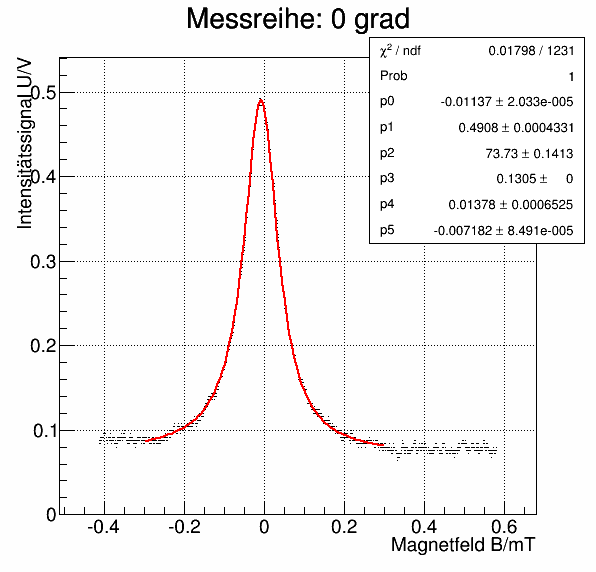
\includegraphics[scale=0.3]{Bilder/0_8}
\caption{$\theta=0^{\circ}$, $T=8^{\circ}C$}
\end{center}
\end{figure}
\clearpage
\begin{figure}[h]
\begin{center}
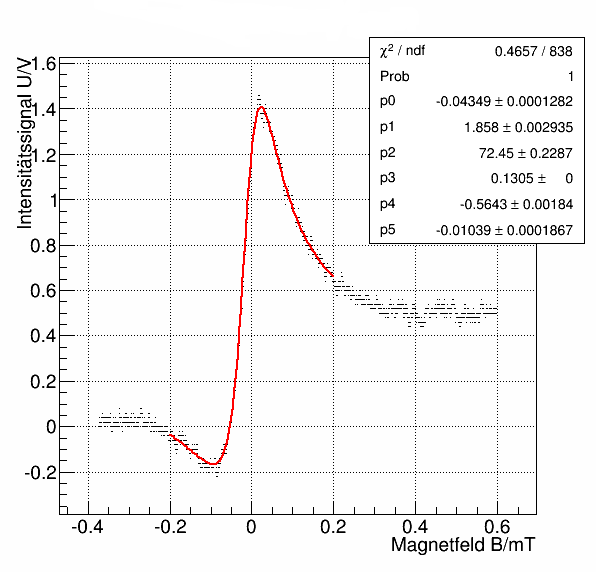
\includegraphics[scale=0.3]{Bilder/45_m4}
\caption{$\theta=45^{\circ}$, $T=-4^{\circ}C$}
\end{center}
\end{figure}
~\\
\begin{figure}[h]
\begin{center}
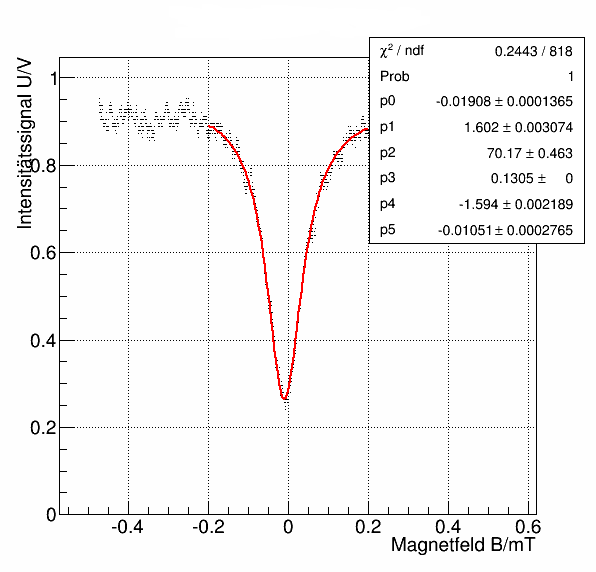
\includegraphics[scale=0.3]{Bilder/90_m6}
\caption{$\theta=90^{\circ}$, $T=-6^{\circ}C$}
\end{center}
\end{figure}
~\\
~\\
Es ist klar zu erkennen, dass die erwarteten Kurvenverläufe bestätigt werden konnten. Es gilt $\frac{\chi^{2}}{Anzahl Freiheitsgrade}<1$, was darauf schließen lässt, dass die Fits sehr gut sind. Dies ist für alle Einstellungen und alle Temperaturen der Fall (siehe Anhang $8.2$).
\subsection{Dampfdruckkurve}
Da, wie bereits im Kapitel 'Theoretische Grundlagen' diskutiert, der Effekt des sog. 'Coherence Narrowing' eliminiert werden soll, muss für die Lebensdauer auf einen Druck von $p=0Pa$ extrapoliert werden. Da nicht der Druck, sondern die Temperatur gemessen wurde, muss diese erst mit der bereits genannten Formel \[ln(p/p_{c})=(T_{c}/T)\cdot\underbrace{(a_{1}T_{r}+a_{2}T_{r}^{1,89}+a_{3}T_{r}^{2}+a_{4}T_{r}^{8}+a_{5}T_{r}^{8,5}+a_{6}T_{r}^{9}}_{:=a})~mit~T_{r}=1-T/T_{C}\]
\[\Leftrightarrow p=p_{c}\cdot e^{\frac{T_{c}}{T}a}\]
Die Werte für die Parameter sind dem Kapitel 'Theoretische Grundlagen' bzw. [ver] zu entnehmen. Für die Temperatur T nahmen wir eine Unsicherheit von $s_{T}=0,5K$ an, da nur in $1K$-Schritten gemessen werden konnte, es allerdings während der Messungen zu keiner Änderung der Anzeige kam. Der Fehler berechnet sich dann zu \[s_{p}=\frac{\partial p}{\partial T}\cdot s_{T}.\] Die erhaltenen Werte sind dem in Anhang $8.3$ vorzufindenden Mathematica-Notebook zu entnehmen.
\subsection{Bestimmung der Lebensdauer}
Um die Lebensdauern zu bestimmen, wurden, wie bereits diskutiert, die aus den Lorentzfits bestimmten Lebensdauern über den Druck aufgetragen und mithilfe eines linearen Fits auf $p=0Pa$ extrapoliert. Der y-Achsenabschnitt gibt die Lebensdauer $\tau$ des angeregten $^{3}P_{1}$-Zustandes von Quecksilber an. 
\subsubsection{Erwärmung}
\begin{figure}[h]
\begin{center}
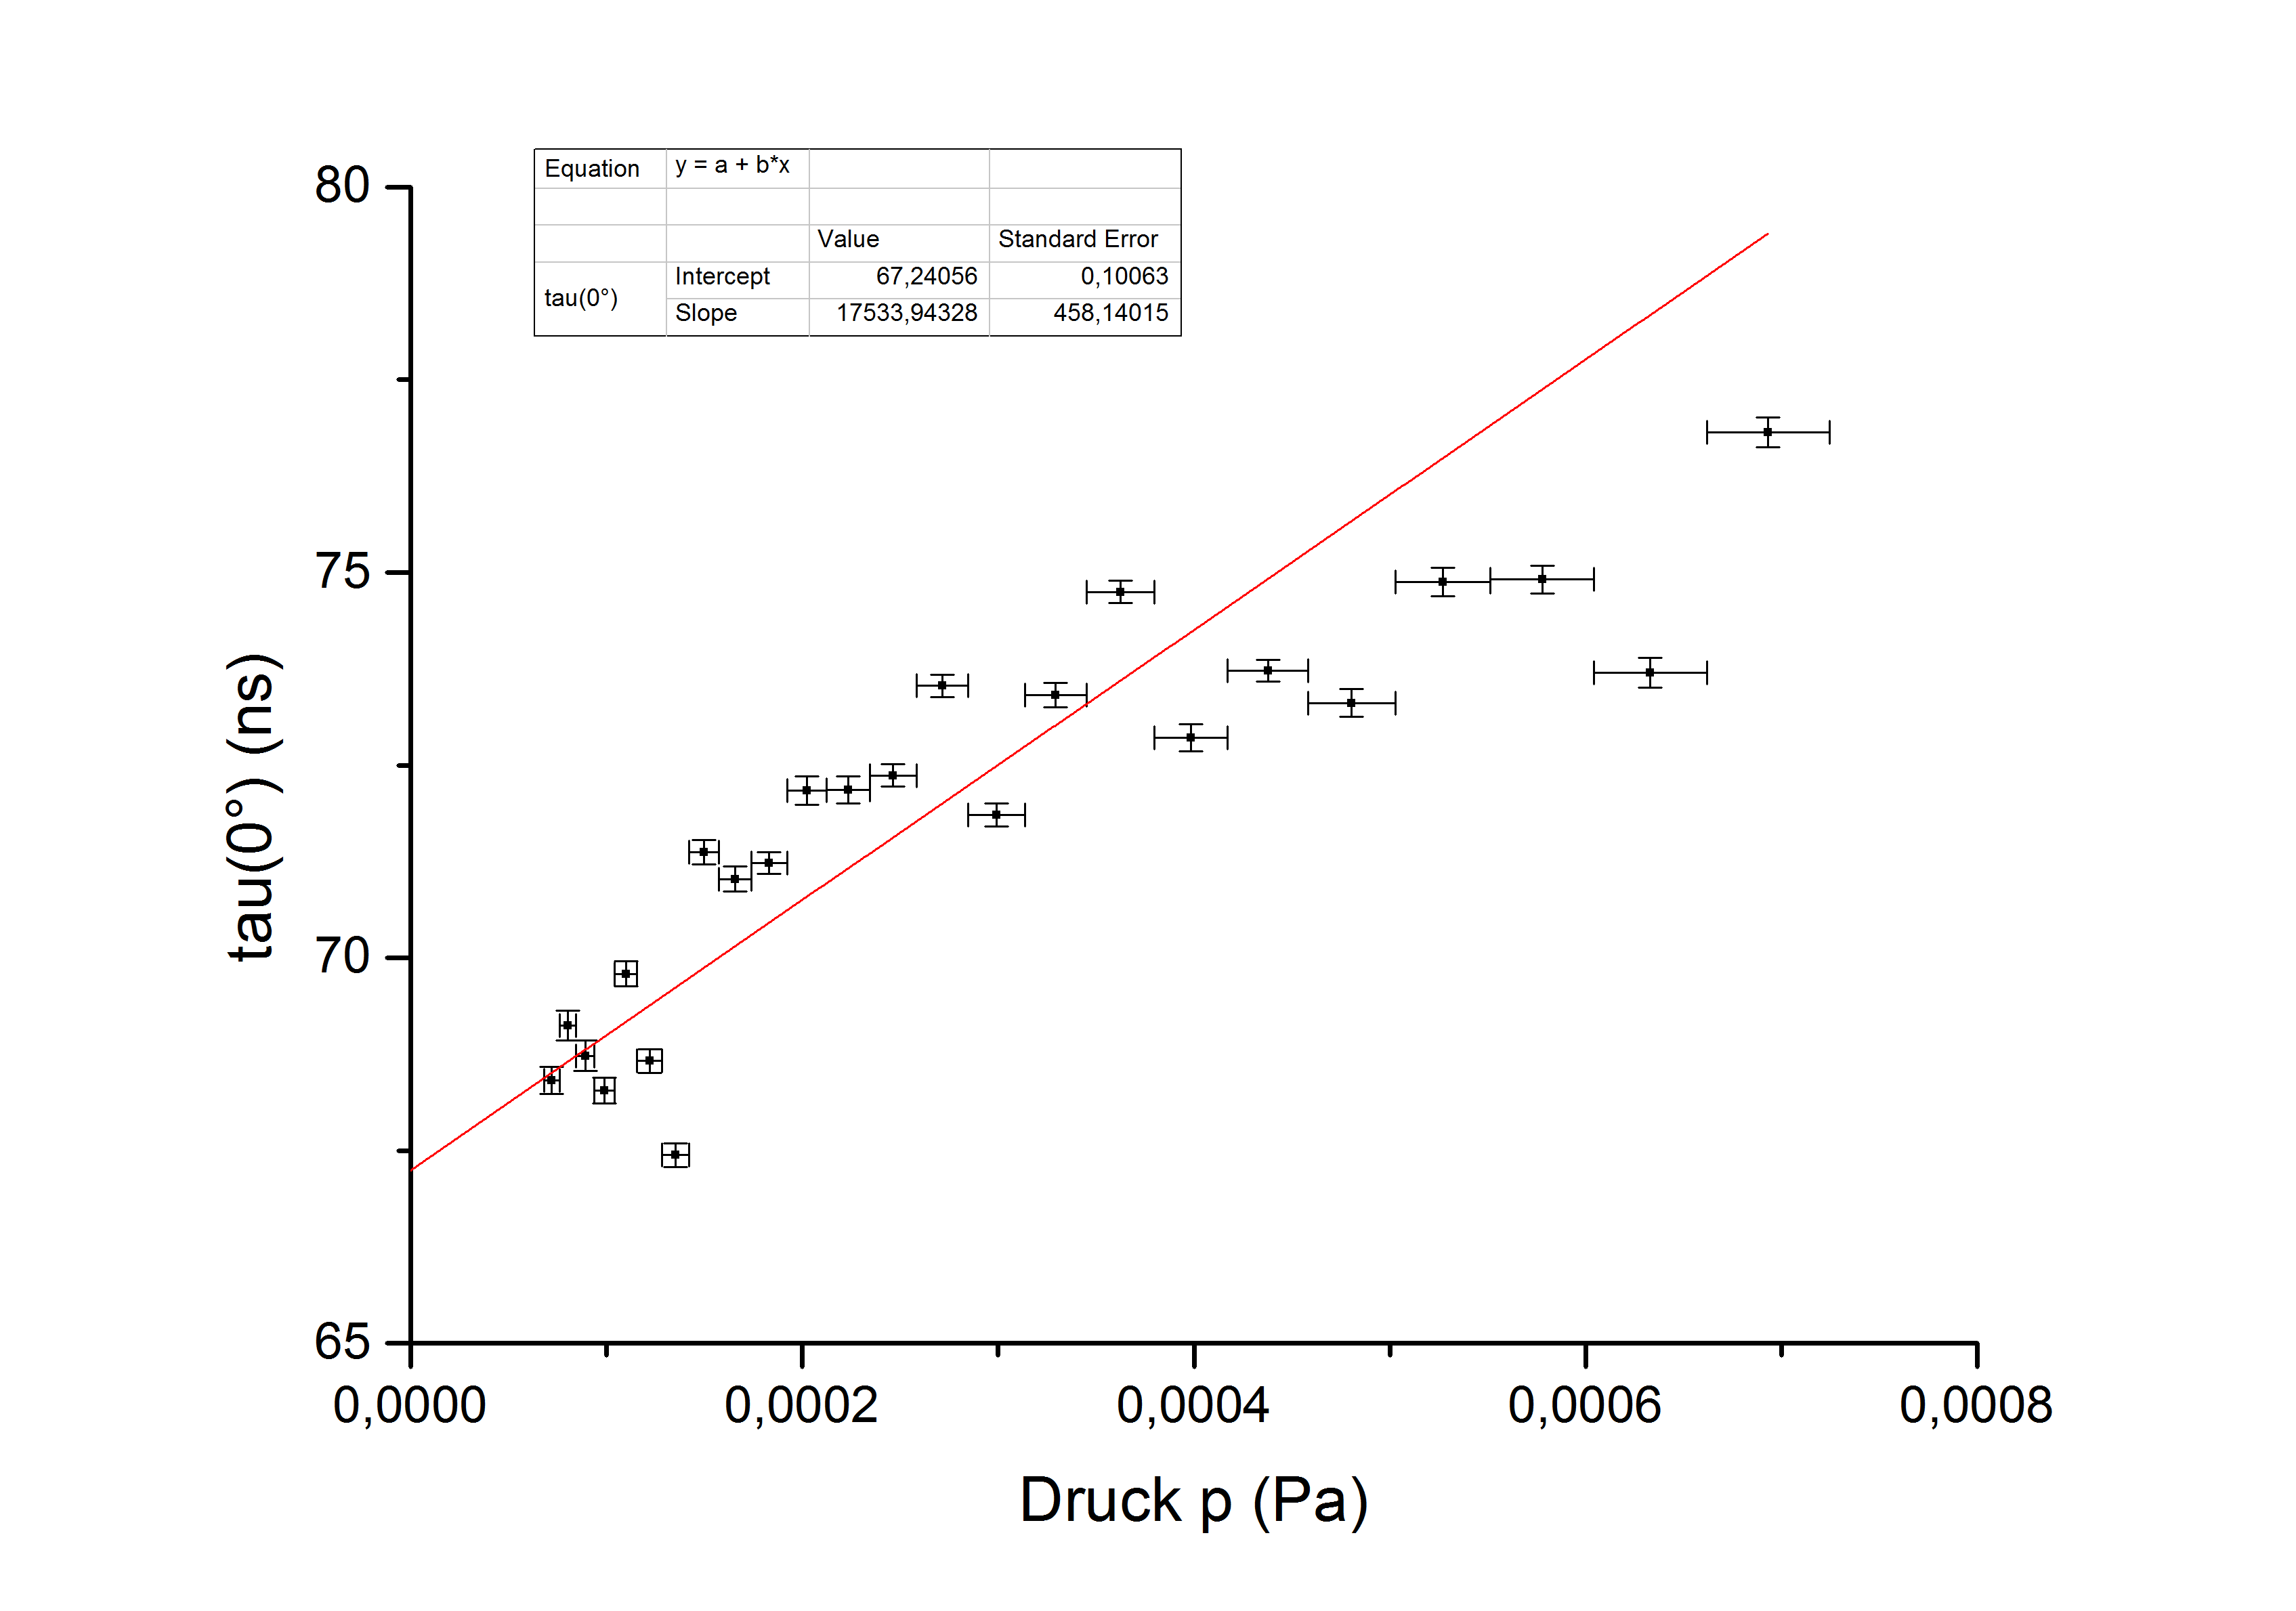
\includegraphics[scale=0.5]{Bilder/erwaermung_0}
\caption{Linearer Fit für $\theta=0^{\circ}$}
\end{center}
\end{figure}
\begin{figure}[h]
\begin{center}
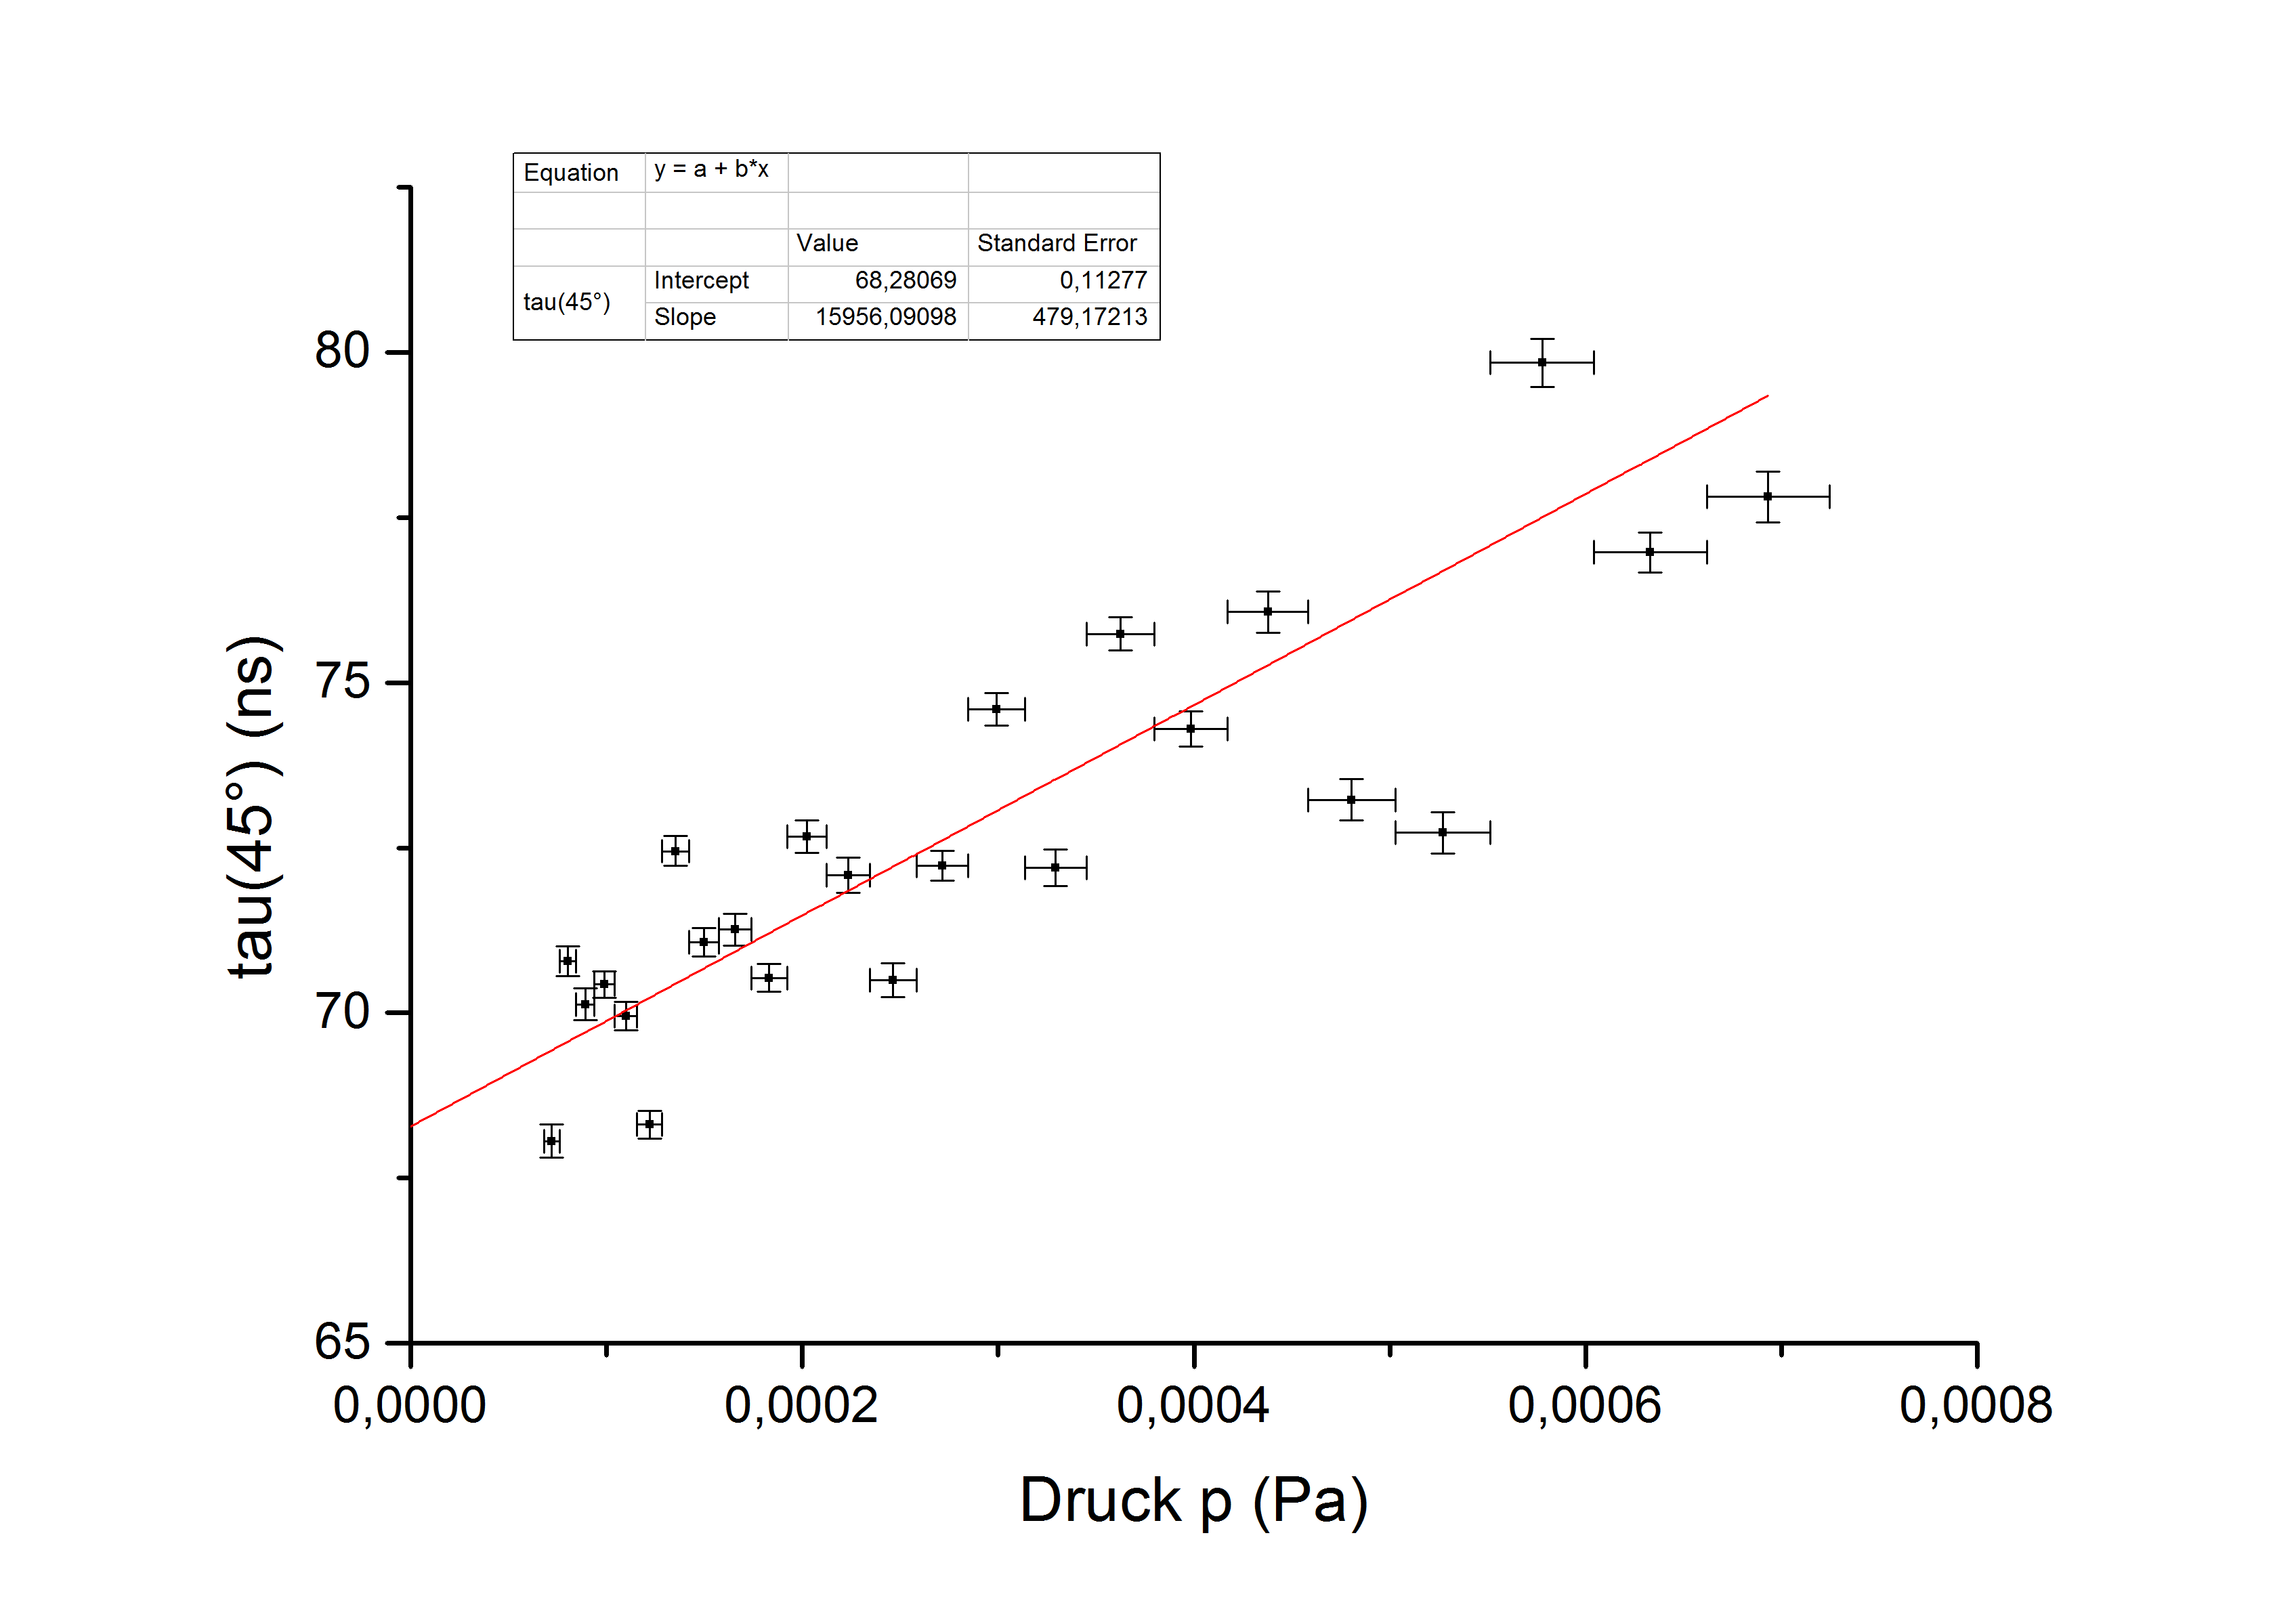
\includegraphics[scale=0.5]{Bilder/erwaermung_45}
\caption{Linearer Fit für $\theta=45^{\circ}$}
\end{center}
\end{figure}
\begin{figure}[h]
\begin{center}
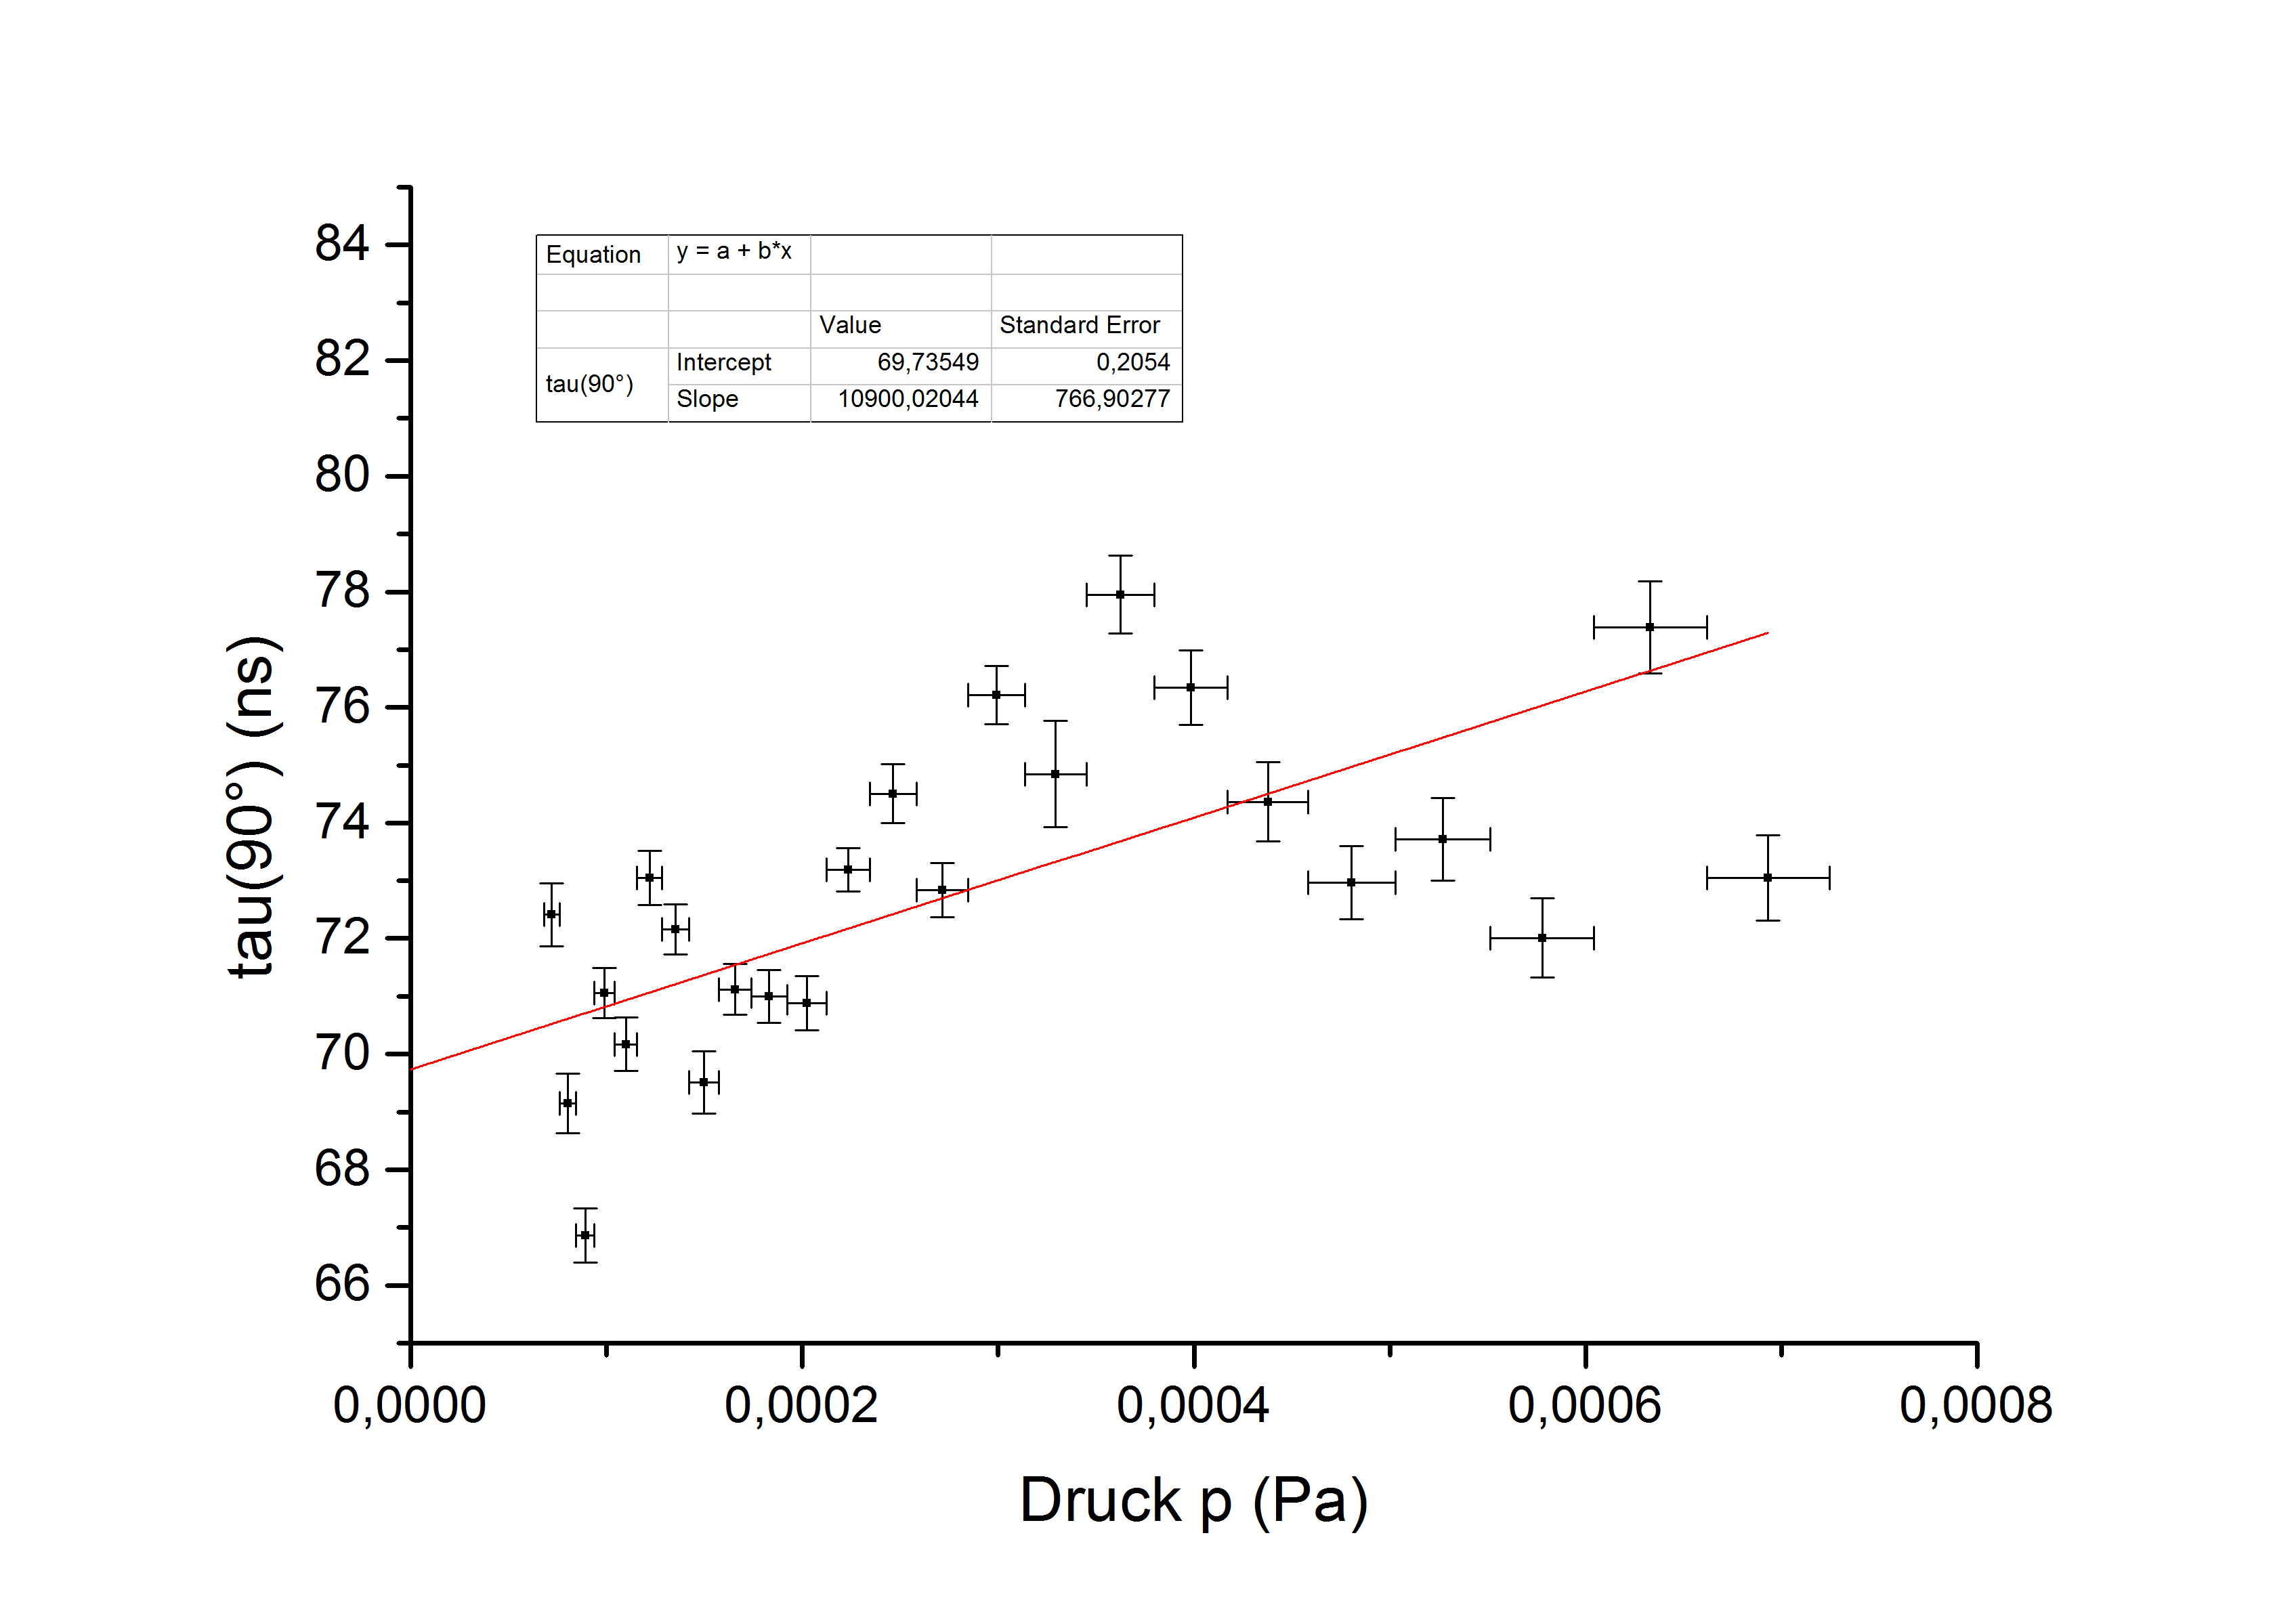
\includegraphics[scale=0.5]{Bilder/erwaermung_90}
\caption{Linearer Fit für $\theta=90^{\circ}$}
\end{center}
\end{figure}
\clearpage
Man erkennt, dass die Werte ziemlich gut durch Geraden gefittet werden konnten. Aufgrund der geringen gemessenen Intensitäten kommt es dabei zu Schwankungen für die $\tau$. Auch statistische Effekte spielen bei der beobachteten Streuung eine Rolle. \\
Für die Lebensdauern erhielten wir:\\
\begin{table}[htbp]
\begin{center}
\caption{}
\begin{tabular}{|r|l|}
\hline
\multicolumn{1}{|l|}{Polarisatoreinstellung $\theta$} & Lebensdauer $\tau$ in ns \\ \hline
$0^{\circ}$ & $(67,24\pm0,10)$ \\ \hline
$45^{\circ}$ & $(68,28\pm0,11)$ \\ \hline
$90^{\circ}$ & $(69,7\pm0,2)$ \\ \hline
\end{tabular}
\end{center}
\label{}
\end{table}
~\\
Da wir stets zunächst eine Messung für den $90^{\circ}$-Winkel, dann für den $45^{\circ}$-Winkel und schließlich für den $0^{\circ}$-Winkel aufnahmen, ist es logisch, dass die Lebensdauer für $\theta=90^{\circ}$ als die größte und diejenige für $\theta=0^{\circ}$ als die kleinste bestimmt wurde, da es sich hier um einen Erwärmungsprozess handelt und somit für den ersteren Winkel der Intensitätsverlauf für eine niedrigere Temperatur und somit einen niedrigeren Druck vermessen wurde. Verschiebt man die Kurve nun zu einem höheren Druck, so erhält man wegen der negativen Steigung des linearen Fits eine niedrigere Lebensdauer, was hier auch beobachtet werden kann. Aus diesem Grund ist auch davon auszugehen, dass die mithilfe des linearen Fits erhaltenen Fehler deutlich zu klein sind, da die Werte im Rahmen der Messungenauigkeit übereinstimmen sollten, was sie hier nicht tun.
\subsubsection{Abkühlung}
\begin{figure}[h]
\begin{center}
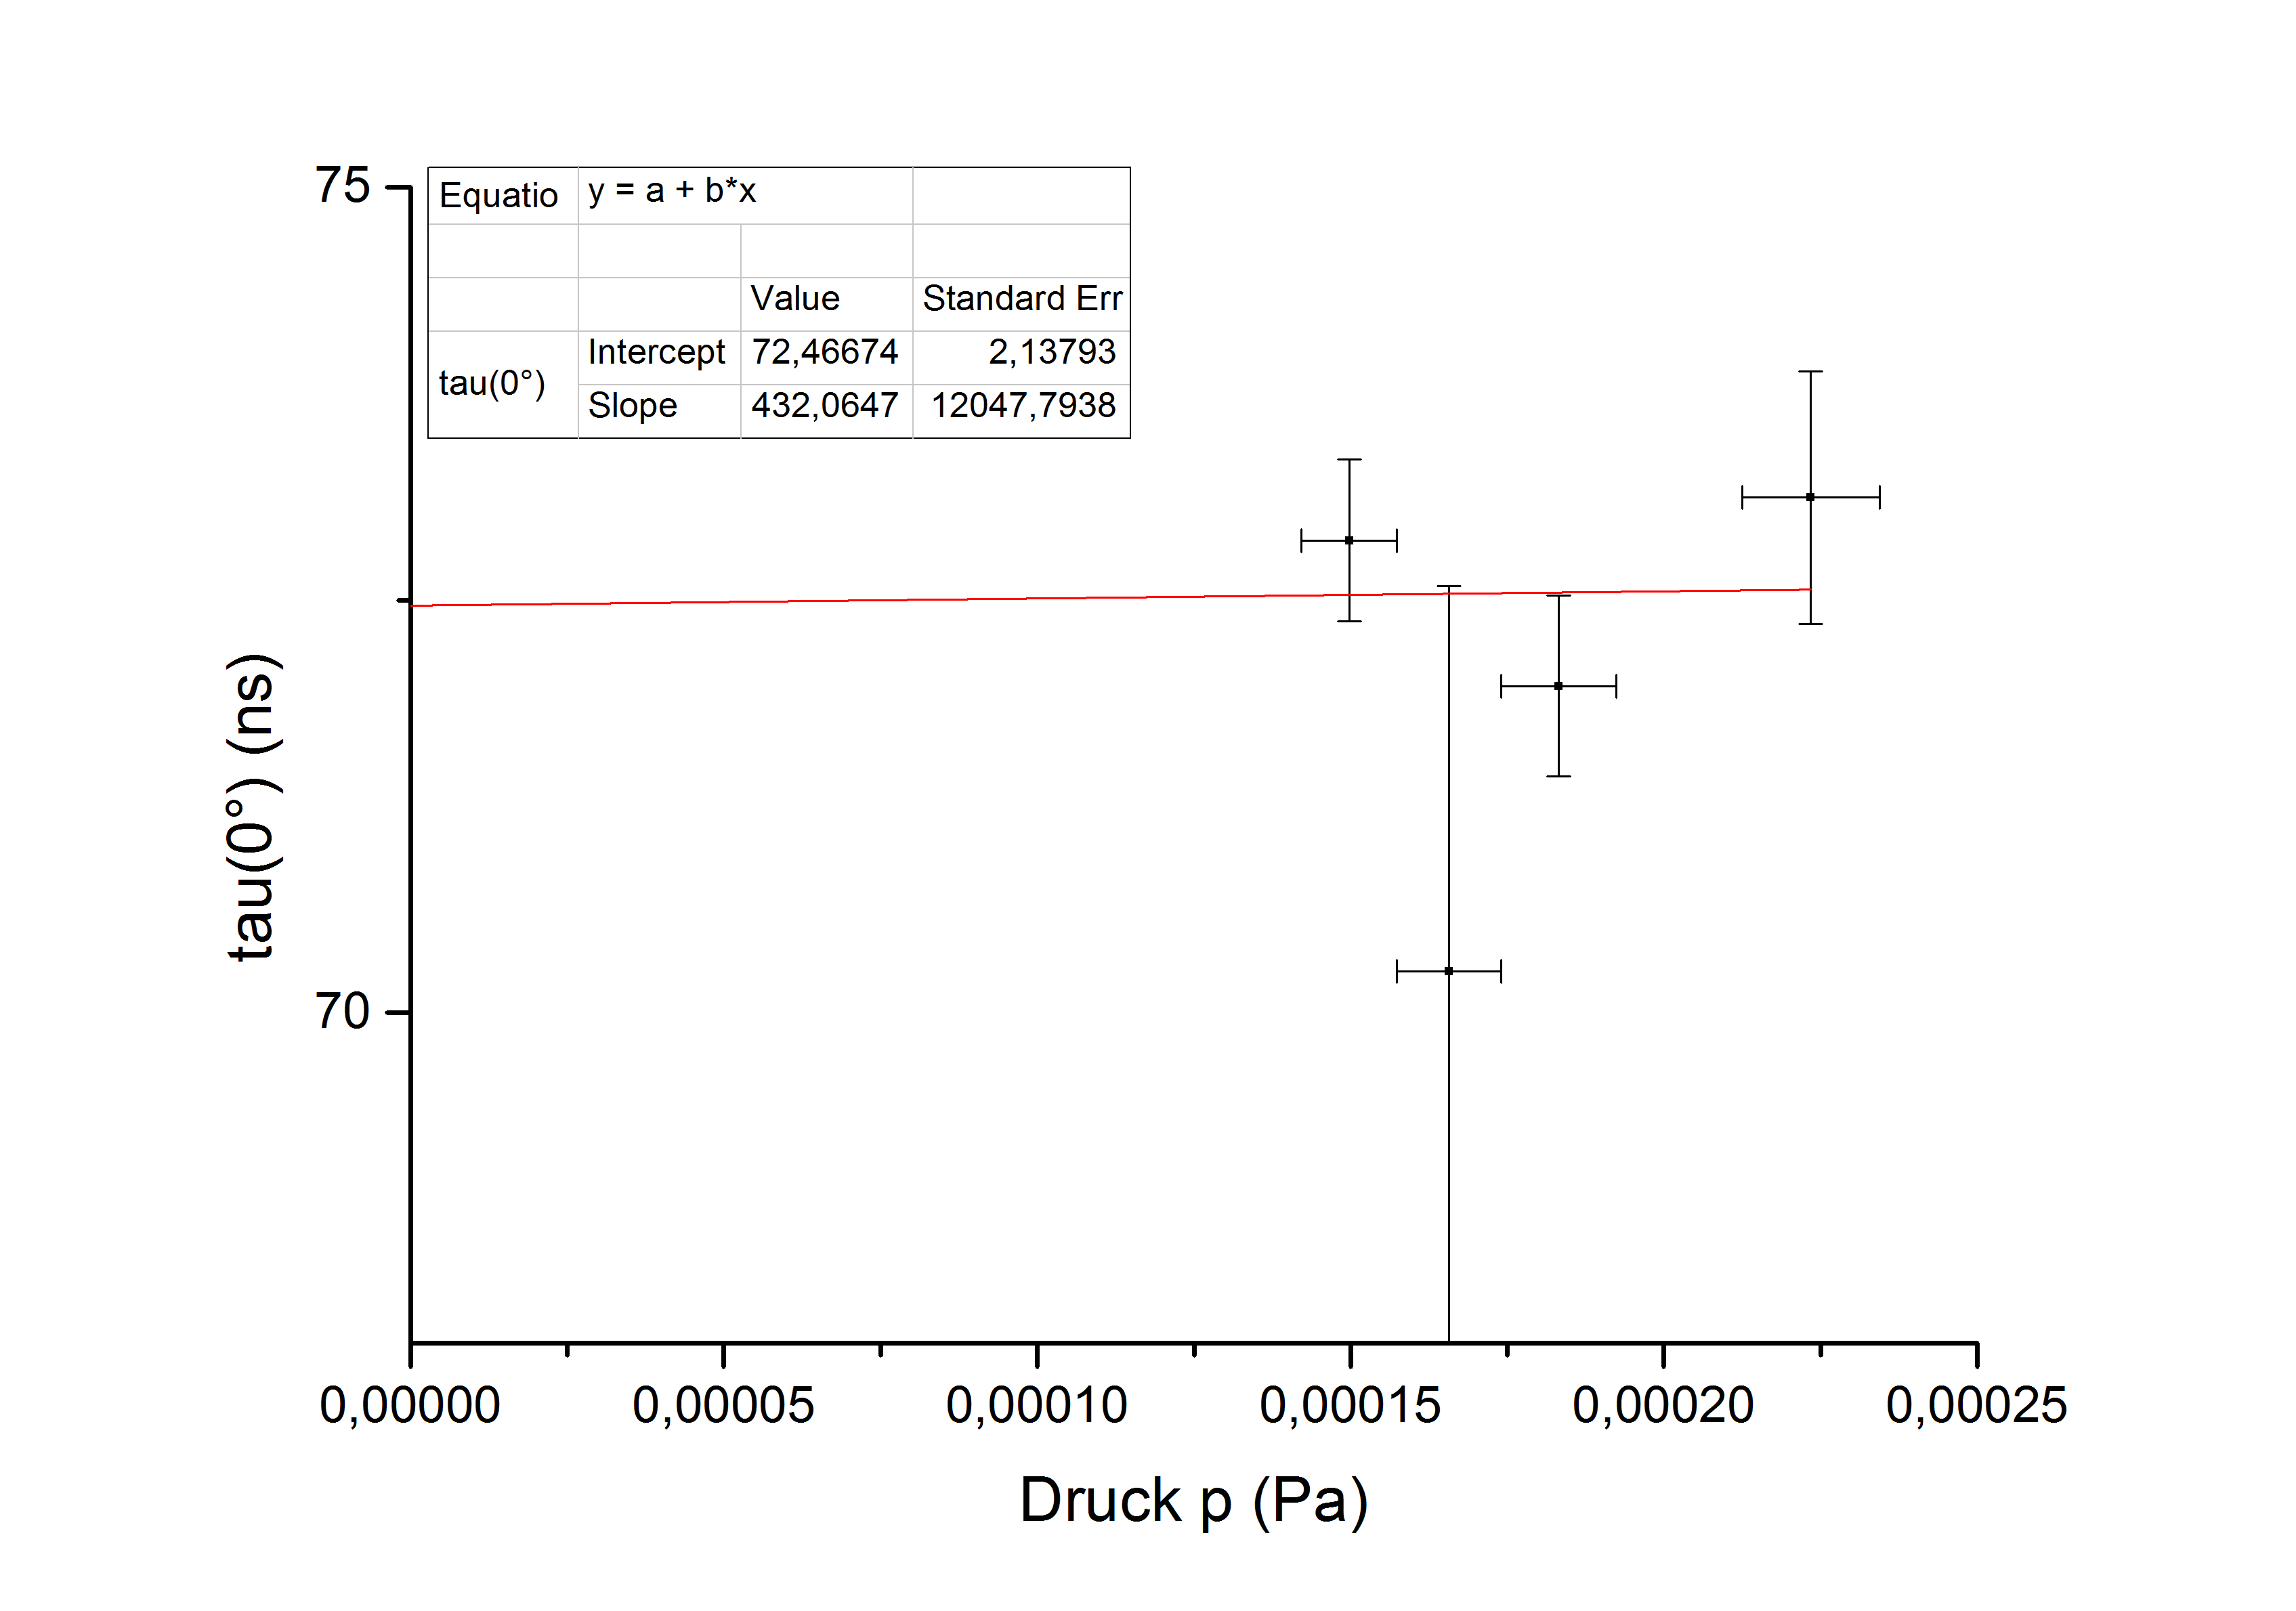
\includegraphics[scale=0.5]{Bilder/abkuehlung_0}
\caption{Linearer Fit für $\theta=0^{\circ}$}
\end{center}
\end{figure}
\begin{figure}[h]
\begin{center}
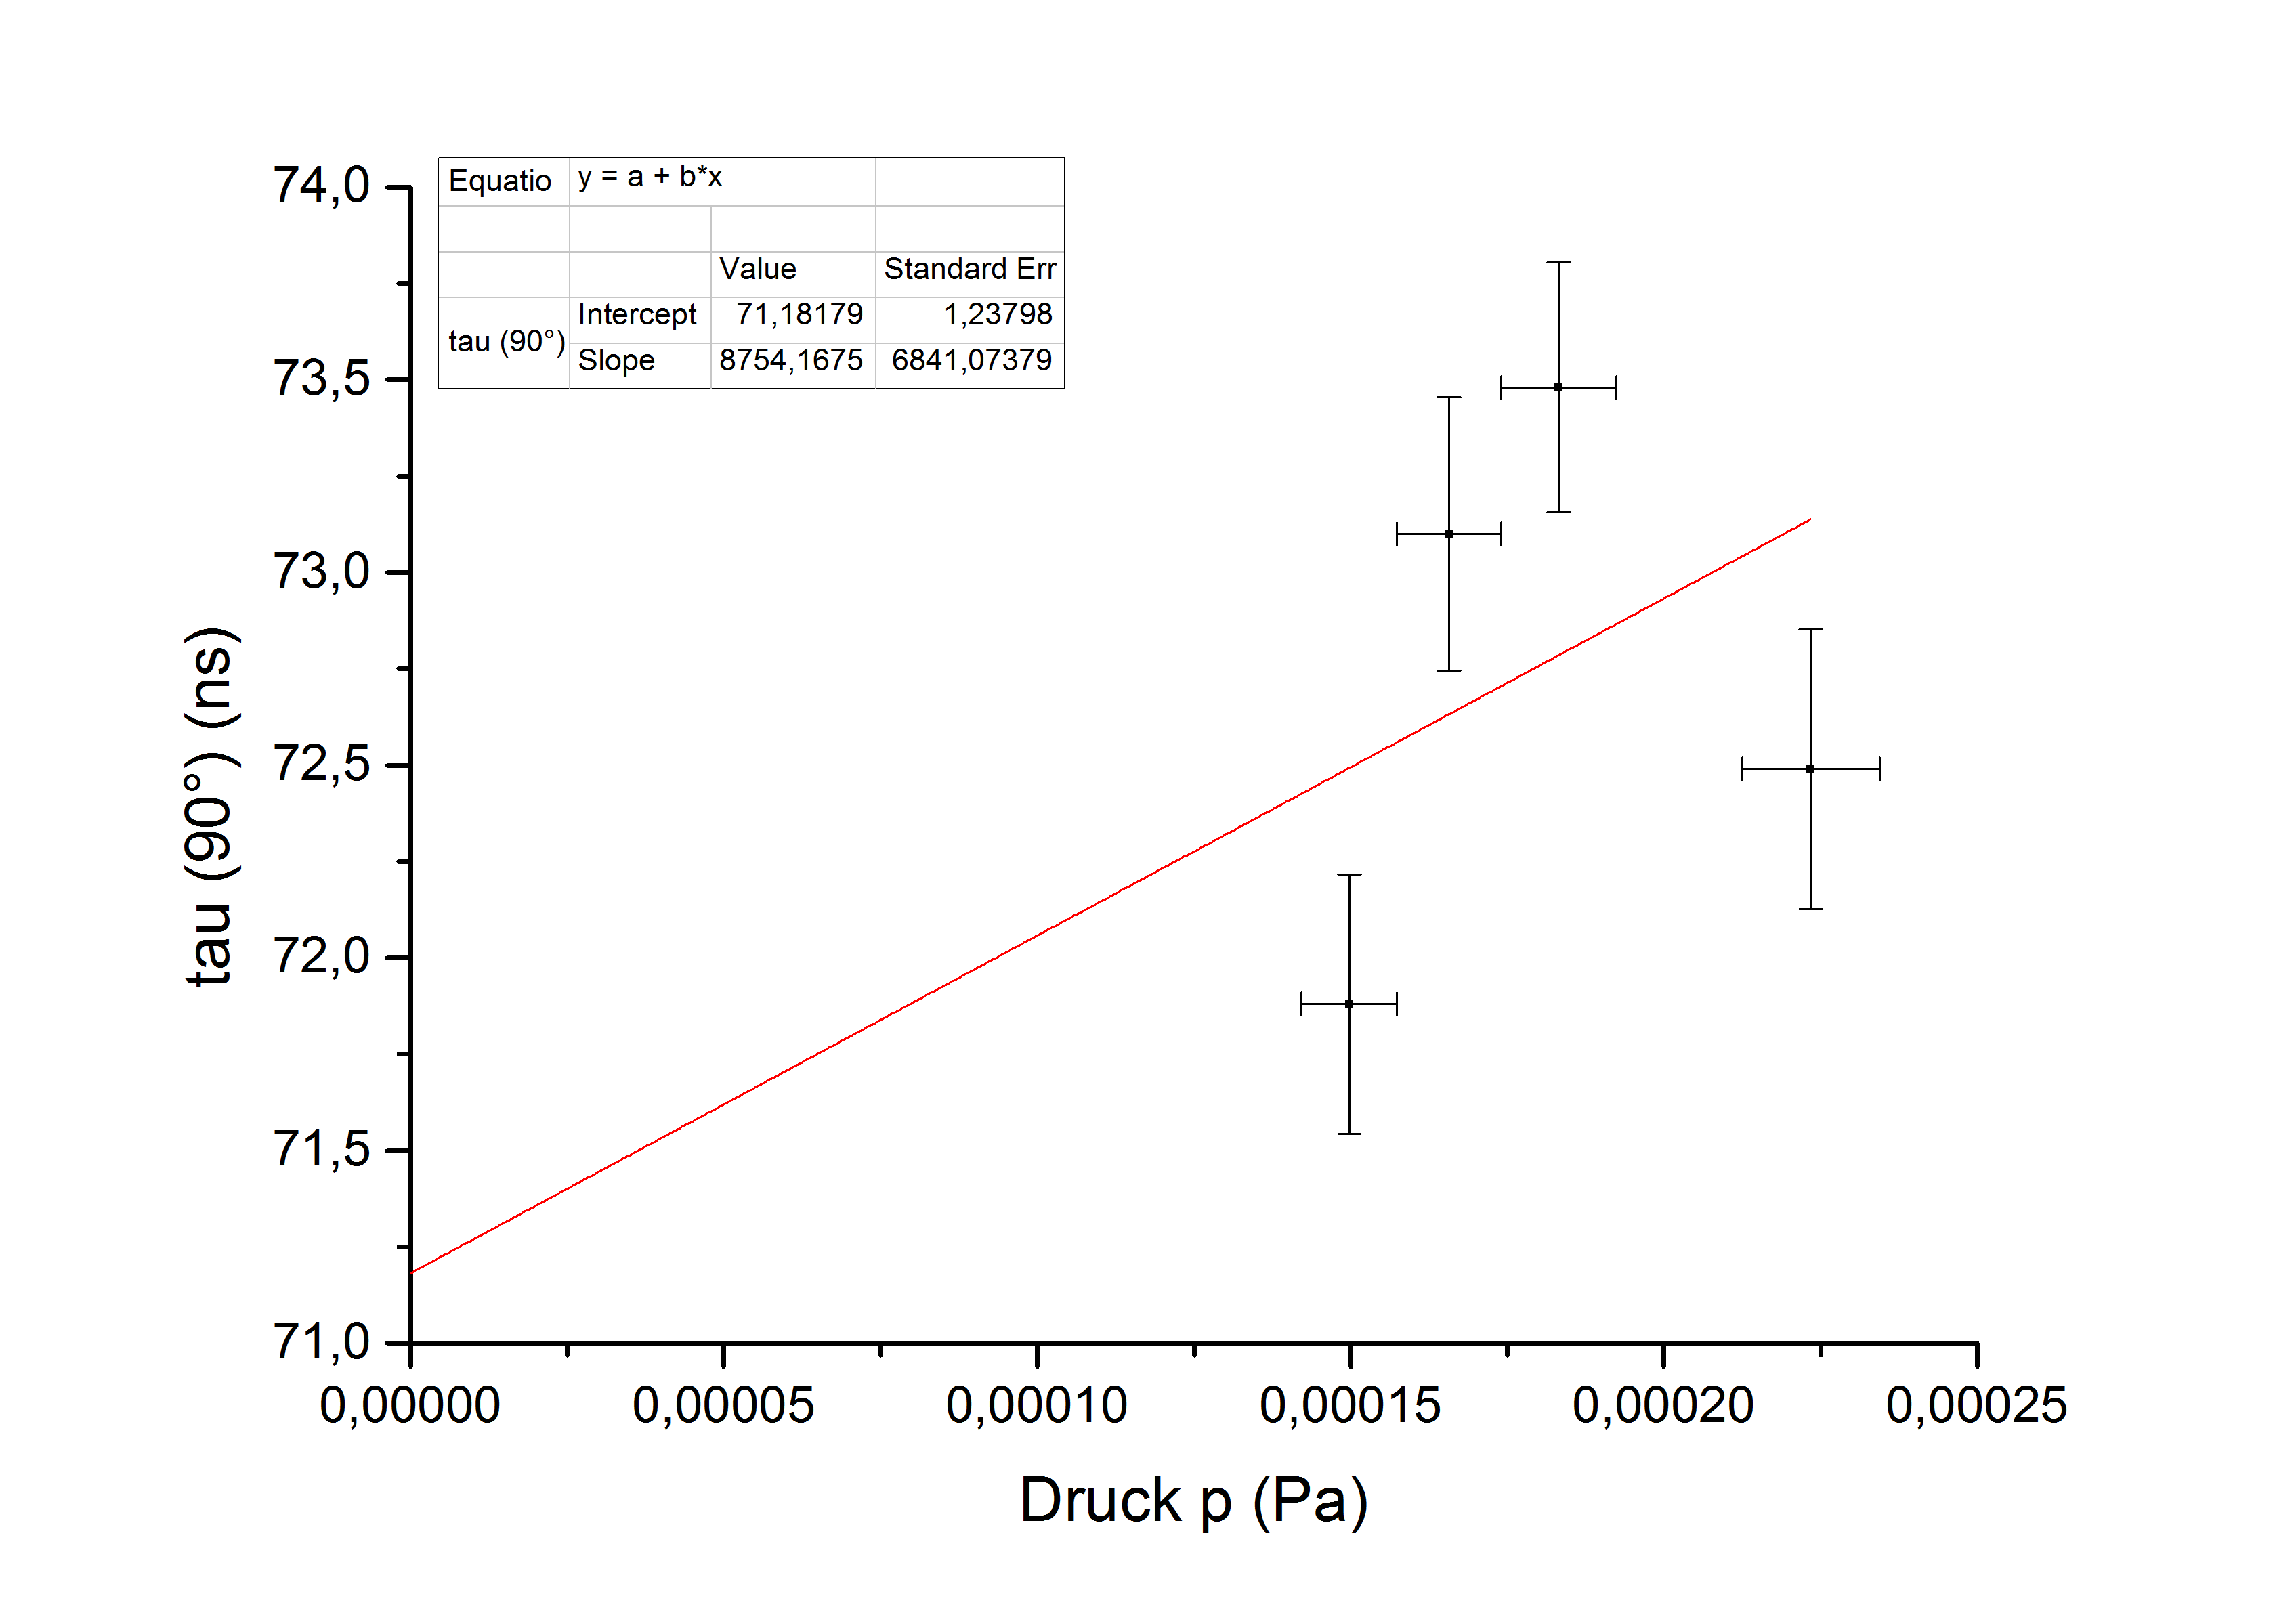
\includegraphics[scale=0.5]{Bilder/abkuehlung_90}
\caption{Linearer Fit für $\theta=90^{\circ}$}
\end{center}
\end{figure}
~\\
~\\
Für die Lebensdauern erhielten wir somit:
\begin{table}[htbp]
\begin{center}
\caption{}
\begin{tabular}{|r|l|}
\hline
\multicolumn{1}{|l|}{Polarisatoreinstellung $\theta$} & Lebensdauer $\tau$ in ns \\ \hline
$0^{\circ}$ & $(72\pm2)$ \\ \hline
$90^{\circ}$ & $(71,2\pm1,2)$ \\ \hline
\end{tabular}
\end{center}
\label{}
\end{table}
~\\
Die erhaltenen Werte im Rahmen der Messungenauigkeit überein, was sich auf die geringere Anzahl an Messungen im Vergleich zur Messreihe für die Erwärmung und den daraus resultierenden größeren Fehler des extrapolierten y-Achsenabschnitts zurückführen lässt. Es ist zu beobachten, dass die Streuung der Werte besonders für $\theta=90^{\circ}$ groß ist. Dies lässt vermuten, dass der Fehler auf $\tau$, welcher nur durch die Standardabweichung mithilfe der Lorentzfits bestimmt wurde, zu gering ist. 
\subsubsection{Fehlerbetrachtung}
Der Literaturwert für die Lebensdauer des $^{3}P_{1}$-Zustandes von Quecksilber beträgt $\tau_{Lit}=119 ns$ (Quelle: [ver]). Es ist klar zu sehen, dass die mithilfe unserer Messungen bestimmten Lebensdauern eine große Abweichung von $\tau_{Lit}$ aufweisen. \\
Eine mögliche Ursache hierfür ist der systematische Fehler, der dadurch gemacht wird, dass der Temperatursensor nicht direkt in der Quarzresonanzzelle, sondern in dem ihn umgebenden Kupferblock angebracht ist, welcher durch die gute Wärmeleitfähigkeit von Kupfer sehr schnell auf Temperaturveränderungen reagiert. Aus diesem Grund ist davon auszugehen, dass die Resonanzzelle bei aufsteigender Temperatur etwas kälter als abgelesen war, bei sinkender Temperatur dagegen etwas wärmer. Aus diesem Grund müsste aufgrund der negativen Steigung der linearen Fits für die Erwärmung (Punkte zu niedrigeren Temperaturen verschoben) die extrapolierte Lebensdauer (der y-Achsenabschnitt) etwas größer sein, für die Abkühlung dagegen etwas kleiner. Tatsächlich erhielten wir, wie in den vorigen Kapiteln zu sehen, leicht höhere Werte für die Lebensdauer mithilfe der Messreihe, bei der die Resonanzzelle abgekühlt wurde, als für die Erwärmung. \\
Es ist aber auch zu sehen, dass die Differenz zwischen den erhaltenen Werten für die Lebensdauer $\tau$ der beiden Messreihen klein ist und somit der eben diskutierte systematische Fehler nicht der Grund für die große Abweichung vom Literaturwert sein kann. Es ist vielmehr wahrscheinlich, dass die äußeren B-Felder nicht richtig kompensiert wurden. Wie bereits erwähnt, hatten wir große Probleme bei der Minimierung des Signals, da die Nadel immer wieder große Schwankungen zeigte, was an externen Störfeldern oder einfach daran liegen kann, dass die Anzeige selbst eine kleine Unsicherheit hat. Dies kann das Ergebnis massiv beeinflussen, da bereits kleine Veränderungen im FWHM eine relativ große Veränderung in der erhaltenen Lebensdauer verursachen können.\\
Möglich ist auch, dass die Einstellung des Polarisators nicht optimal war, was aber aufgrund der Symmetrie der erhaltenen Signale (s. Anhang $8.2$) unwahrscheinlich ist.
\section{Zusammenfassung}
Die Lebensdauern wurden mithilfe von Messungen mit ausgeschalteten (Erwärmung) und angeschalteten Peltier-Elementen (Abkühlung) vermessen. Dabei erhielten wir folgende Ergebnisse:\\
\begin{table}[htbp]
\begin{center}
\caption{Erwärmung}
\begin{tabular}{|r|l|}
\hline
\multicolumn{1}{|l|}{Polarisatoreinstellung $\theta$} & Lebensdauer $\tau$ in ns \\ \hline
$0^{\circ}$ & $(67,24\pm0,10)$ \\ \hline
$45^{\circ}$ & $(68,28\pm0,11)$ \\ \hline
$90^{\circ}$ & $(69,7\pm0,2)$ \\ \hline
\end{tabular}
\end{center}
\label{}
\end{table}
~\\
\begin{table}[htbp]
\begin{center}
\caption{Abkühlung}
\begin{tabular}{|r|l|}
\hline
\multicolumn{1}{|l|}{Polarisatoreinstellung $\theta$} & Lebensdauer $\tau$ in ns \\ \hline
$0^{\circ}$ & $(72\pm2)$ \\ \hline
$90^{\circ}$ & $(71,2\pm1,2)$ \\ \hline
\end{tabular}
\end{center}
\label{}
\end{table}
~\\
Der Literaturwert für den $^{3}P_{1}$-Zustand von Quecksilber beträgt $119 ns$. Es ist klar zu sehen, dass die von uns bestimmten Werte deutlich kleiner als dieser sind. Für eine Diskussion der möglichen Ursachen siehe das Unterkapitel 'Fehlerbetrachtung' im Kapitel 'Auswertung'.
